\chapter{Finding 2: Scheduling Request Deadlock}
\label{ch:m2}

\section{The Scheduling Request Procedure in TS 38.321}
\label{sec:m2proc}

In 5G NR, a UE requires an explicit uplink grant from the gNB before transmitting on the Physical Uplink
Shared Channel (PUSCH). In a legacy handover, the UE executes the Random Access (RACH) procedure; the
gNB responds with Msg2 (Random Access Response), which explicitly provides both uplink timing alignment
and an initial uplink grant.

In contrast, RACH-less LTM intentionally skips the random access handshake. Under TS~38.300
clause~9.2.3.5.1, the UE accesses the target cell via either a configured grant or a dynamic grant, and
begins monitoring PDCCH on the target cell for dynamic scheduling as soon as the switch starts; it may
not trigger random access before the switch completes unless it holds a valid PUCCH resource for the
SR. When dynamic grant scheduling is used, the cell switch command MAC CE can additionally carry an SR
configuration ID pointing the UE to the PUCCH resource for sending that request~\cite{3gpp38300}.
Because pre-allocating dedicated configured grants across all candidate cells is resource-intensive and
optional, standard deployments rely on dynamic scheduling. The UE arrives at the target cell with
no valid uplink grant, forcing it to issue a Scheduling Request (SR)---a 1-bit indicator on
PUCCH Format~0---to request an initial grant to transmit its \texttt{RRCReconfigurationComplete} message.

TS~38.321 clause~5.4.4 governs the SR retry loop~\cite{3gpp38321}. The UE maintains an internal counter
\texttt{SR\_COUNTER}, initialized to zero. For each transmission attempt, the UE increments \texttt{SR\_COUNTER}
and starts \texttt{sr-ProhibitTimer}. If an uplink grant arrives, the procedure terminates successfully.
However, if no grant is received after \texttt{sr-TransMax} attempts, \texttt{SR\_COUNTER} exhausts and
execution falls into the clause's \texttt{else} branch.

\section{The Specification Defect: TS 38.321 Clause 5.4.4}
\label{sec:m2gap}

\Cref{fig:deadlock} illustrates TS~38.321 clause~5.4.4 as a formal condition tree, preserving 3GPP's
normative indentation depths (\texttt{1>} through \texttt{6>}). A critical structural defect exists
in the asymmetric placement of resource teardown versus recovery actions:

\begin{figure}[htbp]
  \centering
  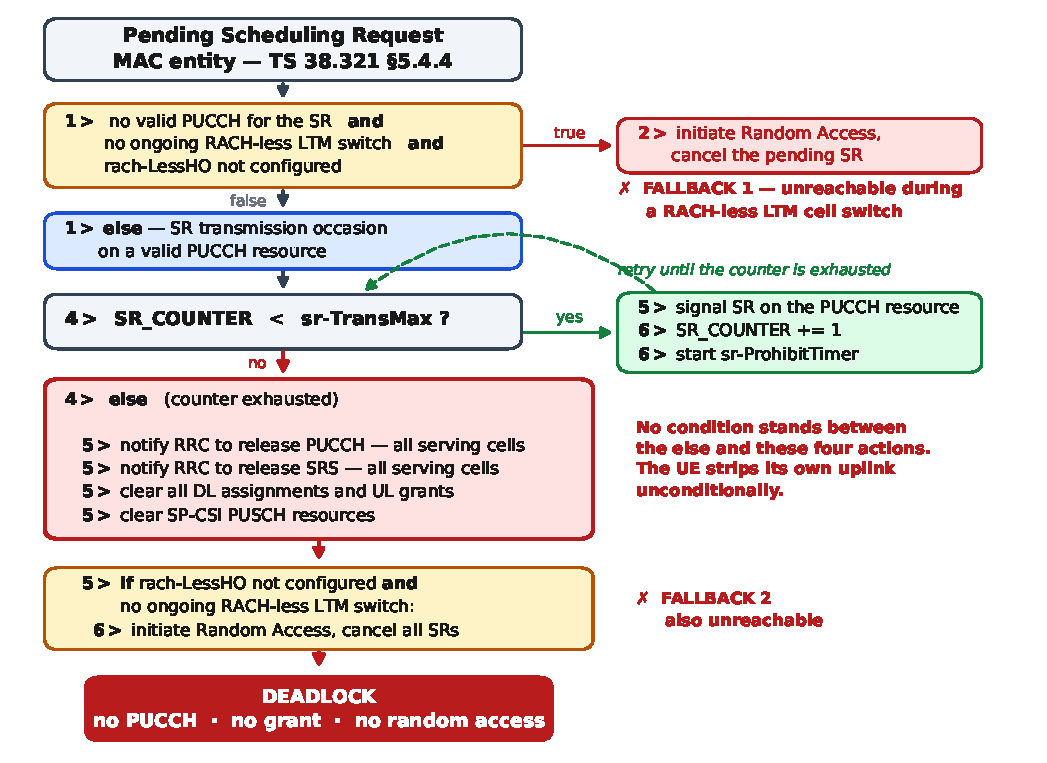
\includegraphics[width=\textwidth]{figures/atk16_deadlock.pdf}
  \caption{Condition tree of TS~38.321 clause~5.4.4. The resource deallocation actions at depth \texttt{5>}
  execute unconditionally on counter exhaustion. The recovery action (initiating Random Access) at depth
  \texttt{6>} is blocked because the guard condition evaluates to false during a RACH-less LTM switch.}
  \label{fig:deadlock}
\end{figure}

\begin{itemize}\itemsep2pt
  \item \textbf{Unconditional Resource Teardown (Depth \texttt{5>}):} When \texttt{SR\_COUNTER} exhausts,
        the specification executes four destructive actions directly beneath the \texttt{else} statement
        with no qualifying conditions, unconditionally stripping the UE of all physical uplink control and
        grant resources: release of PUCCH and SRS for all serving cells, clearing of all configured
        downlink assignments and uplink grants, and clearing of any PUSCH resource for semi-persistent CSI
        reporting---including the very PUCCH channel used to signal scheduling requests.
  \item \textbf{Gated Recovery Path (Depth \texttt{6>}):} The sole action that would restore uplink
        connectivity---initiating random access to recover from the failure---is nested one level deeper,
        conditioned on \texttt{rach-LessHO} being unconfigured and no RACH-less LTM cell switch being
        ongoing; only then does the UE initiate Random Access (clause~5.1) on the SpCell and cancel all
        pending SRs.
\end{itemize}

During an ongoing RACH-less LTM switch, the second conjunct is \textbf{false}. Consequently, the recovery
action at depth \texttt{6>} is completely skipped. Furthermore, the clause's alternative path to random
access (taken if no valid PUCCH resource is configured) is guarded by the identical condition.

\paragraph{Protocol Deadlock:} The UE loses every UE-initiated path back to uplink connectivity:
\begin{enumerate}\itemsep1pt
  \item It holds no uplink grants and no PUCCH resources to request new grants.
  \item The only mechanism capable of allocating new resources on its own initiative (Random Access) is
        explicitly forbidden.
  \item The blocking condition, an ongoing RACH-less LTM cell switch, cannot clear, because cell-switch
        completion requires transmitting an RRC reconfiguration complete message, which is impossible
        without an uplink grant.
\end{enumerate}
The same clause~9.2.3.5.1 keeps the UE monitoring PDCCH for a dynamic grant throughout
(\cref{sec:m2proc}), so the bare defect is not strictly permanent on its own; \cref{sec:m2dyngrant} shows
why the attack closes that escape anyway.

\section{The Attack: Forcing Deadlock via Corrupted Timing Advance}
\label{sec:m2threat}

While the deadlock defect exists as an inherent specification flaw, reaching counter exhaustion by chance
under normal radio conditions is vanishingly rare ($P \approx 10^{-12}$). However, an adversary leverages
the corrupted candidate \TA{} from Finding~1 to drive the UE into this deadlock deterministically.

\subsection{Attack Execution}
The attack proceeds in five deterministic steps:
\begin{enumerate}\itemsep2pt
  \item \textbf{Preamble Delay Injection:} During candidate cell early acquisition, the adversary's RF
        relay intercepts the UE's preamble and forwards it with $\Delta \ge 7\,T_{\mathrm{unit}}$ excess
        delay. The candidate gNB computes an inflated \TA{} and forwards it to the serving gNB via F1AP.
  \item \textbf{RACH-less Handover Trigger:} The serving gNB issues an LTM Cell Switch Command MAC CE
        containing this corrupted \TA{}. Because a \TA{} is present, TS~38.300 mandates a RACH-less switch.
        The UE applies the bad \TA{} and skips random access.
  \item \textbf{PUCCH SR Decorrelation:} Arriving at the target cell with no grant, the UE transmits an
        SR on the PUCCH resource indicated by the switch command. Because its transmit timing is
        misaligned by $\ge 7\,T_{\mathrm{unit}}$, the gNB detector's coherent phase correlation across
        subcarriers collapses completely. The target gNB cannot decode the SR.
  \item \textbf{Deterministic Counter Exhaustion:} The UE retransmits the SR at every periodic occasion.
        Because the timing error is static and persistent, every subsequent SR attempt fails with high
        probability. \texttt{SR\_COUNTER} reaches \texttt{sr-TransMax} with near certainty under flat
        fading ($P \ge 0.996$ at 7 units) and with high probability under multipath ($P = 0.75$--$0.97$,
        \cref{tab:determinism}).
  \item \textbf{Deadlock:} Clause 5.4.4 executes the \texttt{else} branch, releasing PUCCH, SRS, and all
        grants. Because the switch is RACH-less, random access is blocked. The UE is silenced; whether it
        stays silenced is addressed in \cref{sec:m2dyngrant}.
\end{enumerate}

\begin{table}[htbp]
  \centering
  \caption{Comparison of SR counter exhaustion by random channel fading versus corrupted \TA{} attack
  at $\texttt{sr-TransMax}=8$, 10\,dB SNR, 1 receive port.}
  \label{tab:determinism}
  \small
  \begin{tabularx}{\textwidth}{@{}l X r r@{}}
    \toprule
    Timing Condition & Channel Environment & Per-Attempt Loss & $P(\text{Exhaustion})$ \\
    \midrule
    \multicolumn{4}{@{}l}{\textbf{Honest UE (Aligned \TA{})}} \\
    Synchronized ($\Delta_{\mathrm{TA}} = 0$) & Flat Rayleigh fading & 0.0365 & $3.0 \times 10^{-12}$ \\
    Synchronized ($\Delta_{\mathrm{TA}} = 0$) & Additive White Gaussian Noise & $<0.0005$ & $\ll 10^{-9}$ \\
    \midrule
    \multicolumn{4}{@{}l}{\textbf{Adversary-Corrupted \TA{} Attack}} \\
    Error $\Delta_{\mathrm{TA}} = 6$ units & Flat Rayleigh fading & 0.9720 & $0.797$ \\
    Error $\Delta_{\mathrm{TA}} = 7$ units & Flat Rayleigh fading & 0.9995 & $0.996$ \\
    Error $\Delta_{\mathrm{TA}} = 7$ units & Urban Multipath Profile & 0.9650 & $0.750$ \\
    Error $\Delta_{\mathrm{TA}} = 8$ units & Urban Multipath Profile & 0.9965 & $0.970$ \\
    Error $\Delta_{\mathrm{TA}} \ge 8$ units & AWGN / Flat fading & 1.0000 & $1.000$ \\
    \bottomrule
  \end{tabularx}
\end{table}

\subsection{Why the Trigger is Deterministic}
As shown in \cref{tab:determinism}, random channel errors result in independent Bernoulli trials,
yielding an exhaustion probability of $0.0365^8 \approx 3 \times 10^{-12}$. In contrast, a timing
advance error of $\ge 7$ units creates correlated, structural failures: every transmission
arrives misaligned. The per-attempt loss probability reaches $0.9995$, driving the probability of
deadlock to $0.996$ under flat fading and $0.970$ under multipath (at 8 units).

\subsection{The Dynamic Grant Does Not Save the UE}
\label{sec:m2dyngrant}
TS~38.300 clause~9.2.3.5.1 lets the gNB schedule the UE on PDCCH without waiting for an SR, so the bare
specification defect is not, by itself, permanent---a grant the UE never requested would still restore
it. Under the attack, this escape closes twice over. First, any grant the gNB issues still has to be
used on the same misaligned uplink timing: a PUSCH transmission suffers the identical $\ge 7$-unit
offset as the SR did, so it is no more decodable than the request that triggered it. Second, the gNB
has no reason to issue a grant in the first place: it has received nothing from this UE since the
switch began, and an SR-silenced UE is, from the network's side, indistinguishable from an idle one
that has nothing to send. The deadlock is therefore not unbreakable in principle, but the same
corruption that causes it also removes the one practical way out.

\section{Formal Model of Counter Exhaustion and Parameter Space Sweep}
\label{sec:m2model}

Reaching deadlock depends on a race between the time required to exhaust \texttt{SR\_COUNTER}
($T_{\text{exhaust}}$) and the mobility supervision timer \texttt{t304}. The time to exhaustion is:
\begin{equation}
  T_{\text{exhaust}} = \texttt{sr-TransMax} \times T_{\text{interval}},
  \quad
  T_{\text{interval}} = \max\!\left(P_{\mathrm{ms}},\
    \left\lceil \frac{\texttt{sr-ProhibitTimer}}{P_{\mathrm{ms}}} \right\rceil P_{\mathrm{ms}} \right),
  \label{eq:exhaust}
\end{equation}
where $P_{\mathrm{ms}} = P / 2^{\mu}$ represents the SR resource periodicity in milliseconds, and
$T_{\text{interval}}$ accounts for the quantization of \texttt{sr-ProhibitTimer} onto available SR occasions.

\paragraph{State Transition and Deadlock Logic of TS~38.321 Clause~5.4.4:}
The procedural flow of the MAC entity upon SR counter exhaustion proceeds as follows:
\begin{enumerate}\itemsep1pt
  \item \textbf{Periodic Transmission Phase:} At each valid SR occasion spaced by $T_{\text{interval}}$ (\cref{eq:exhaust}), the UE transmits an SR on PUCCH Format~0 and increments \texttt{SR\_COUNTER}.
  \item \textbf{Supervision Timer Race:} If the handover supervision timer \texttt{t304} expires before \texttt{SR\_COUNTER} reaches \texttt{sr-TransMax} ($t \ge \texttt{t304}$), the UE declares handover failure and initiates standard RRC connection re-establishment.
  \item \textbf{Unconditional Teardown (Depth 5>):} When $\texttt{SR\_COUNTER} \ge \texttt{sr-TransMax}$, the MAC entity unconditionally executes:
    \begin{itemize}\itemsep0pt
      \item Notify RRC to release PUCCH and SRS for all serving cells;
      \item Clear any configured downlink assignments and uplink grants;
      \item Clear any semi-persistent CSI reporting resources.
    \end{itemize}
  \item \textbf{Recovery Evaluation (Depth 6>):} The MAC entity evaluates the guard condition for recovery:
    \begin{itemize}\itemsep0pt
      \item \textbf{Legacy / Non-LTM Handover:} If \texttt{rach-LessHO} is not configured, the condition evaluates to true; the UE initiates a Random Access procedure on the target cell to recover.
      \item \textbf{RACH-less LTM Switch:} Because an ongoing RACH-less LTM switch is active, the guard condition strictly evaluates to false. The UE is forbidden from initiating Random Access.
    \end{itemize}
  \item \textbf{Protocol Deadlock State:} With all uplink transmission resources torn down and Random Access recovery inhibited, the UE has no remaining UE-initiated path back to uplink connectivity and is silenced for the remaining duration $T_{\text{dead}} = \texttt{t304} - T_{\text{exhaust}}$, until \texttt{t304} eventually expires. A network-issued dynamic grant remains possible on paper (\cref{sec:m2proc}); \cref{sec:m2dyngrant} shows why it does not materialize in practice, making the dead state effectively unbreakable until timeout.
\end{enumerate}

\subsection{Parameter Space Enumeration (5400 Configurations)}
\label{sec:m2space}
3GPP specifications define parameters via formal ASN.1 definitions in TS~38.331~\cite{3gpp38331}:
\begin{itemize}\itemsep1pt
  \item \texttt{sr-TransMax}: 5 legal values ($\{n4, n8, n16, n32, n64\}$).
  \item \texttt{sr-ProhibitTimer}: 18 legal values (8 Rel-15 values, absent $=0$, plus 9 Rel-17 values).
  \item SR periodicity $P$: 15 legal values ($\{sym2, sym7, sl1, sl2, sl4, \dots, sl640\}$).
  \item Numerology $\mu$: 4 values ($\mu \in \{0, 1, 2, 3\}$).
\end{itemize}
This establishes a finite space of $5 \times 18 \times 15 \times 4 = 5400$ valid 3GPP configurations.
Evaluating this state transition logic across all 5400 configurations reveals that when no LTM switch is ongoing, 100\%
of configurations safely recover via random access. However, during a RACH-less LTM switch, between
\textbf{9.0\% and 77.4\%} of configurations reach this effectively-unbreakable dead state (\cref{sec:m2dyngrant}).

\section{Outage Cost and Timer Interaction}
\label{sec:m2cost}

When deadlock occurs, the UE remains silenced for an outage duration
$T_{\text{dead}} = \texttt{t304} - T_{\text{exhaust}}$ until the supervision timer \texttt{t304} expires.
During $T_{\text{dead}}$, the UE can neither transmit data nor request resources.

\paragraph{Why Radio Link Failure (T310) Does Not Intervene:} One might expect the radio link failure
timer T310 to rescue the UE. It cannot, for two reasons: (i) T310 monitors downlink PDCCH block
error rate, which remains healthy; and (ii) TS~38.331 clause~5.3.5.4 mandates that applying the
\texttt{ReconfigurationWithSync} information element (which starts T304) explicitly stops T310.

\paragraph{Evidence from Clause 5.2 (Conditional LTM Comparison):}
The decisive proof that this defect represents a specification omission appears in TS~38.321 clause~5.2
(governing \texttt{timeAlignmentTimer} expiry)~\cite{3gpp38321}: when a RACH-less CLTM cell switch is
ongoing, the clause branches to initiate Random Access (clause~5.1) on the SpCell; only its \texttt{else}
branch releases PUCCH and SRS and clears grants without that escape. 3GPP therefore already recognized
that a UE losing resources during a RACH-less switch requires an escape to random access, and added it
for Conditional LTM. However, 3GPP omitted this identical remedy from clause~5.4.4 for plain LTM.
Re-inserting this escape into clause~5.4.4 forms the core of our proposed 3GPP remediation.
